%% LyX 2.3.4.4 created this file.  For more info, see http://www.lyx.org/.
%% Do not edit unless you really know what you are doing.
\documentclass[american]{beamer}
\usepackage[T1]{fontenc}
\usepackage[latin9]{inputenc}
\setcounter{secnumdepth}{3}
\setcounter{tocdepth}{3}
\usepackage{amssymb}
\usepackage{graphicx}


\usepackage{babel}
\begin{document}
\title{A model of random walk with varying transition probabilities}
\maketitle
\begin{frame}{Outline}

\begin{enumerate}
\item<1-> {\Large{}Motivation}\bigskip{}
\item<2-> {\Large{}Model description}\bigskip{}
\item<3-> {\Large{}Model application}
\end{enumerate}
\end{frame}
%
\begin{frame}{Random walk}

\begin{definition}
A man starts from a point $O$ and walks $l$ yards in a straight
line;
he then turns through any angle whatever and walks another $l$
yards in a second straight line.
He repeats this process $n$ times.
I require the probability that after these $n$ stretches he is at
a distance between $r$ and $r+\delta r$ from his starting point,
$O.$

{\footnotesize{}\medskip{}
}\emph{\footnotesize{}{[}Karl Pearson: The problem of the random walk.
(1905){]}}{\footnotesize\par}

\begin{description}
\item<2-> [{Where}] is the \emph{``Drunken sailor''}?
\end{description}
\end{definition}

\end{frame}
%
\begin{frame}{Motivation}
\begin{itemize}
\item Failure of a machine
\begin{itemize}
\item repair after failure
\item preventive maintenance
\end{itemize}
\item Occcurence of a disease
\begin{itemize}
\item cure of the disease
\item prevention (i.e. lifestyle change)
\end{itemize}
\item Development of sports match
\begin{itemize}
\item goal scored, point achieved
\item period won
\end{itemize}
\end{itemize}
\end{frame}
%
\begin{frame}{Random walk with varying probabilities}
\begin{itemize}
\item Random walk with memory
\item Memory coefficient $\lambda\in(0,\,1)$ affecting the transition probabilities
\item First step of the walk $X_{1}$ depends on an initial transition probability
$p_{0}$
\item Further steps depending on a transition probability $p_{t}$ evolving
as
\[
X_{t-1}=1\rightarrow p_{t}=\lambda p_{t-1}
\]
\[
X_{t-1}=-1\rightarrow p_{t}=1-\lambda(1-p_{t-1})
\]

\begin{itemize}
\item<1-> ``Success punished''
\[
X_{t-1}=1\rightarrow p_{t}=1-\lambda(1-p_{t-1})
\]
\[
X_{t-1}=-1\rightarrow p_{t}=\lambda p_{t-1}
\]
\item<1-> ``Success rewarded
\end{itemize}
\end{itemize}
\end{frame}
%
\begin{frame}{Formal definition}
\begin{definition}
Let $\ensuremath{p_{0},\lambda\in(0,\,1)}$\textrm{ be constant parameters,
${\{P_{n}\}}_{n=0}^{\infty}$ and ${\{X_{n}\}}_{n=1}^{\infty}$ sequences
of discrete random variables with $P_{0}=p_{0}$ and for $t\ge1$
\[
P(X_{t}=1|P_{t-1}=p_{t-1})=p_{t-1},\,\,\,P(X_{t}=-1|P_{t-1}=p_{t-1})=1-p_{t-1},
\]
and (}\emph{success punishing)}\textrm{
\[
P_{t}=\lambda P_{t-1}+\frac{1}{2}(1-\lambda)(1-X_{t})
\]
or (}\emph{success rewarding)
\[
P_{t}=\lambda P_{t-1}+\frac{1}{2}(1-\lambda)(1+X_{t}).
\]
}The sequence ${\{S_{n}\}}{}_{n=0}^{\infty},\;S_{N}=S_{0}+\sum_{i=1}^{N}X_{i}$
for $n\in\mathbb{N}$, with $S_{0}\in\mathbb{R}$ some given starting
position, is called a \emph{random walk with varying probabilities},
with ${\{X_{n}\}}_{n=1}^{\infty}$ being the steps of the walker and
${\{P_{n}\}}_{n=0}^{\infty}$ transition probabilities. Depending
on the chosen formula to calculate $P_{i}$ the walk type is either
\emph{success punishing} or \emph{success rewarding}.
\end{definition}

\end{frame}
%
\begin{frame}{Example - RW development}

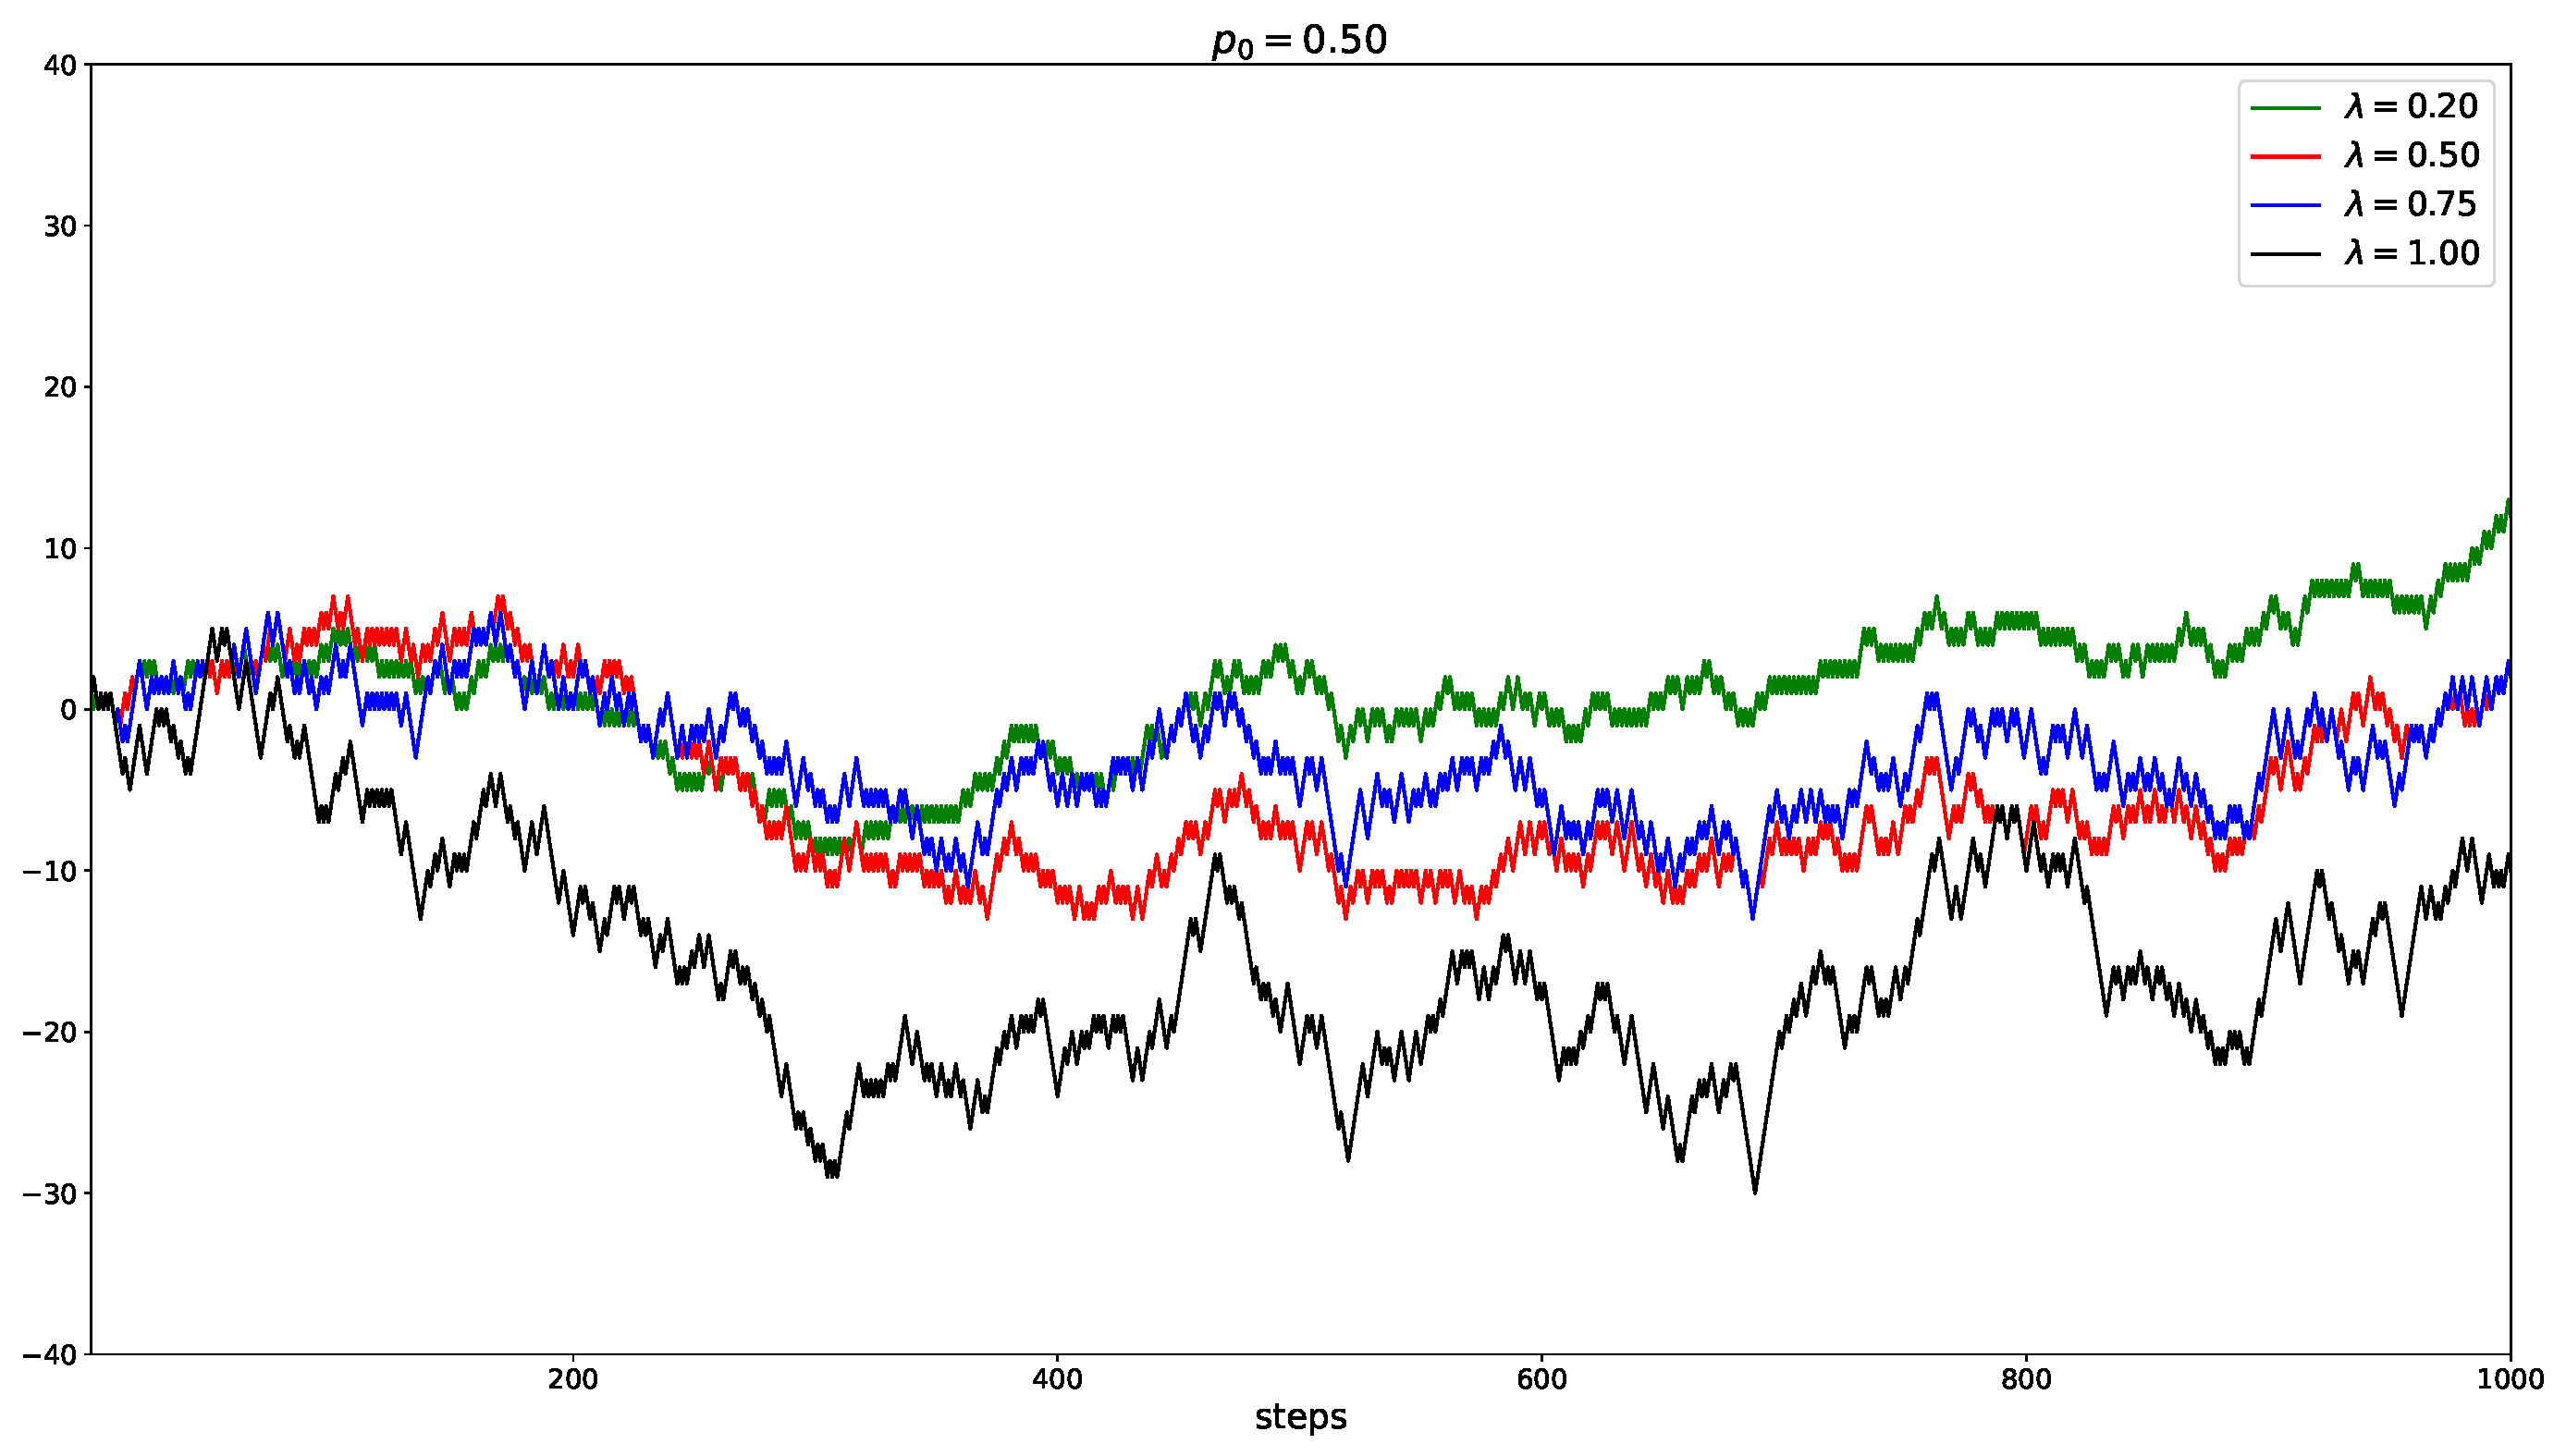
\includegraphics[width=1\textwidth]{../../simulations/single_walk_1000_steps_type_success_punished}

\end{frame}
%
\begin{frame}{Example - RW development}

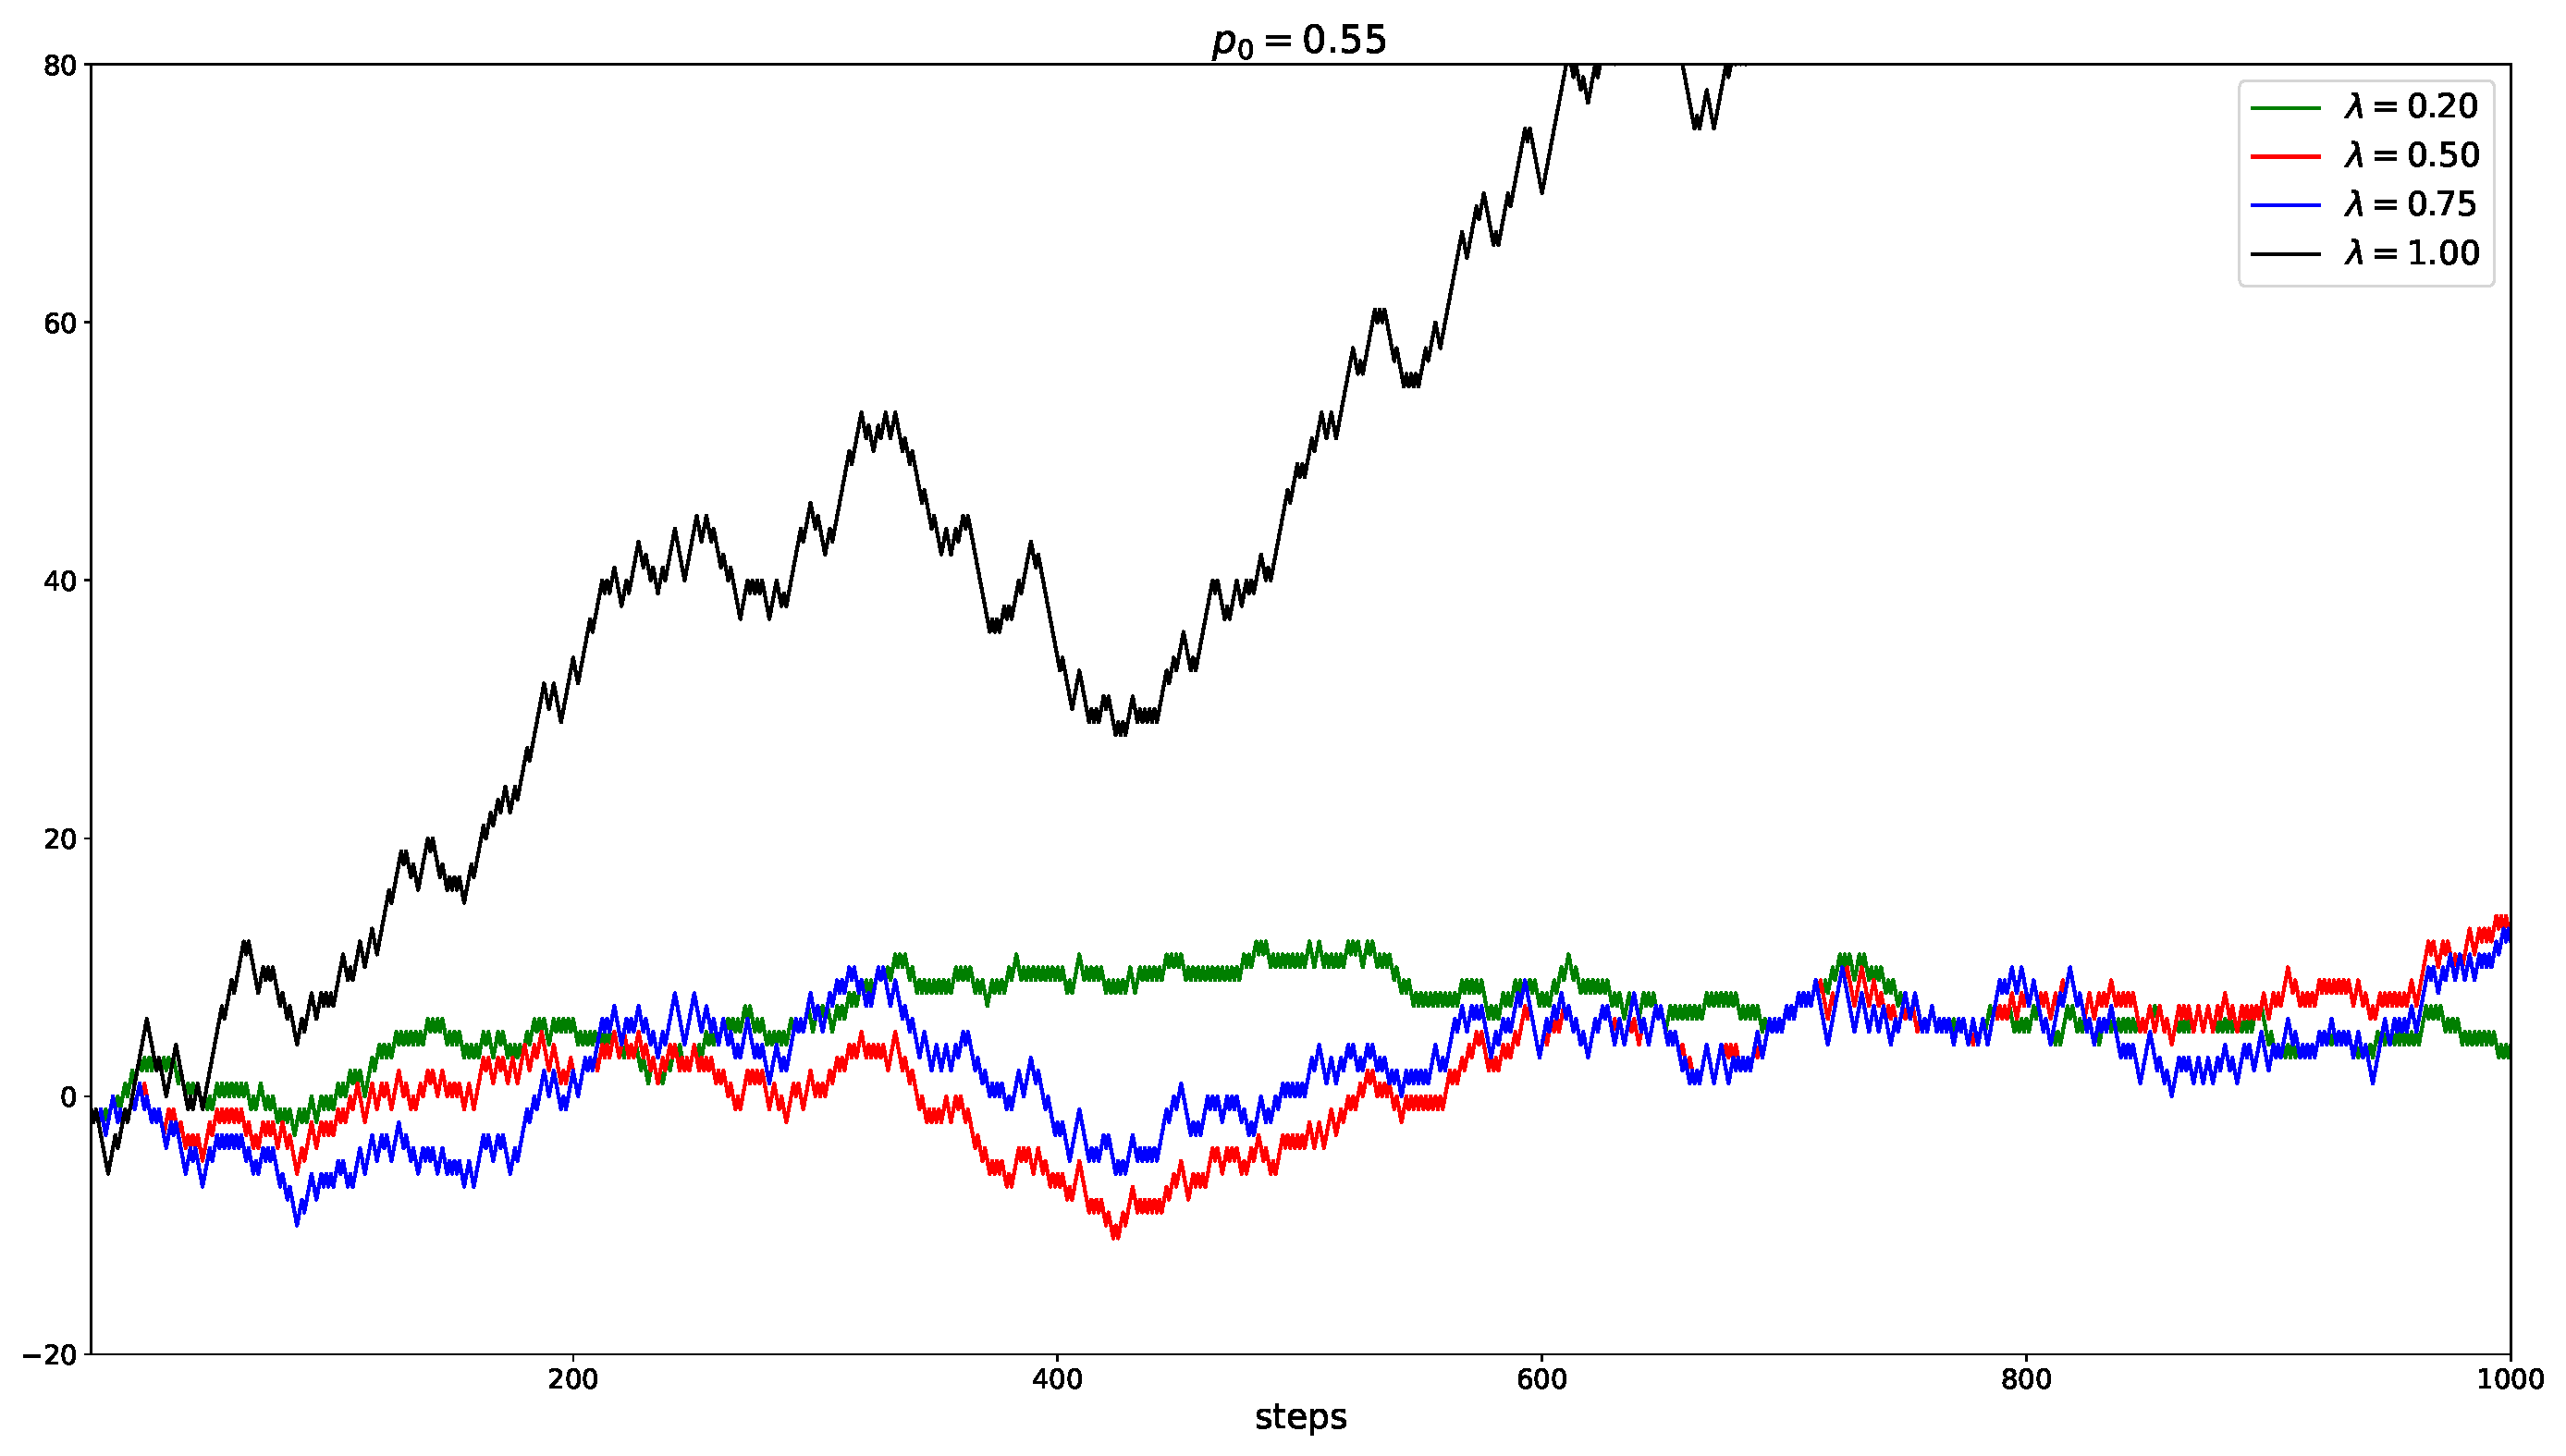
\includegraphics[width=1\textwidth]{../../simulations/single_walk_1000_steps_type_success_punished_p0_0.55}

\end{frame}
%
\begin{frame}{Walk steps properties}

\[
EX_{t}=(2\lambda-1)^{t-1}(2p_{0}-1),
\]
\[
\lim_{t\to+\infty}EX_{t}=0.
\]
\[
Var\,X_{t}=1-(2\lambda-1)^{2(t-1)}(2p_{0}-1)^{2},
\]
\[
\lim_{t\to+\infty}Var\,X_{t}=1.
\]

\end{frame}
%
\begin{frame}{Example - RW steps}

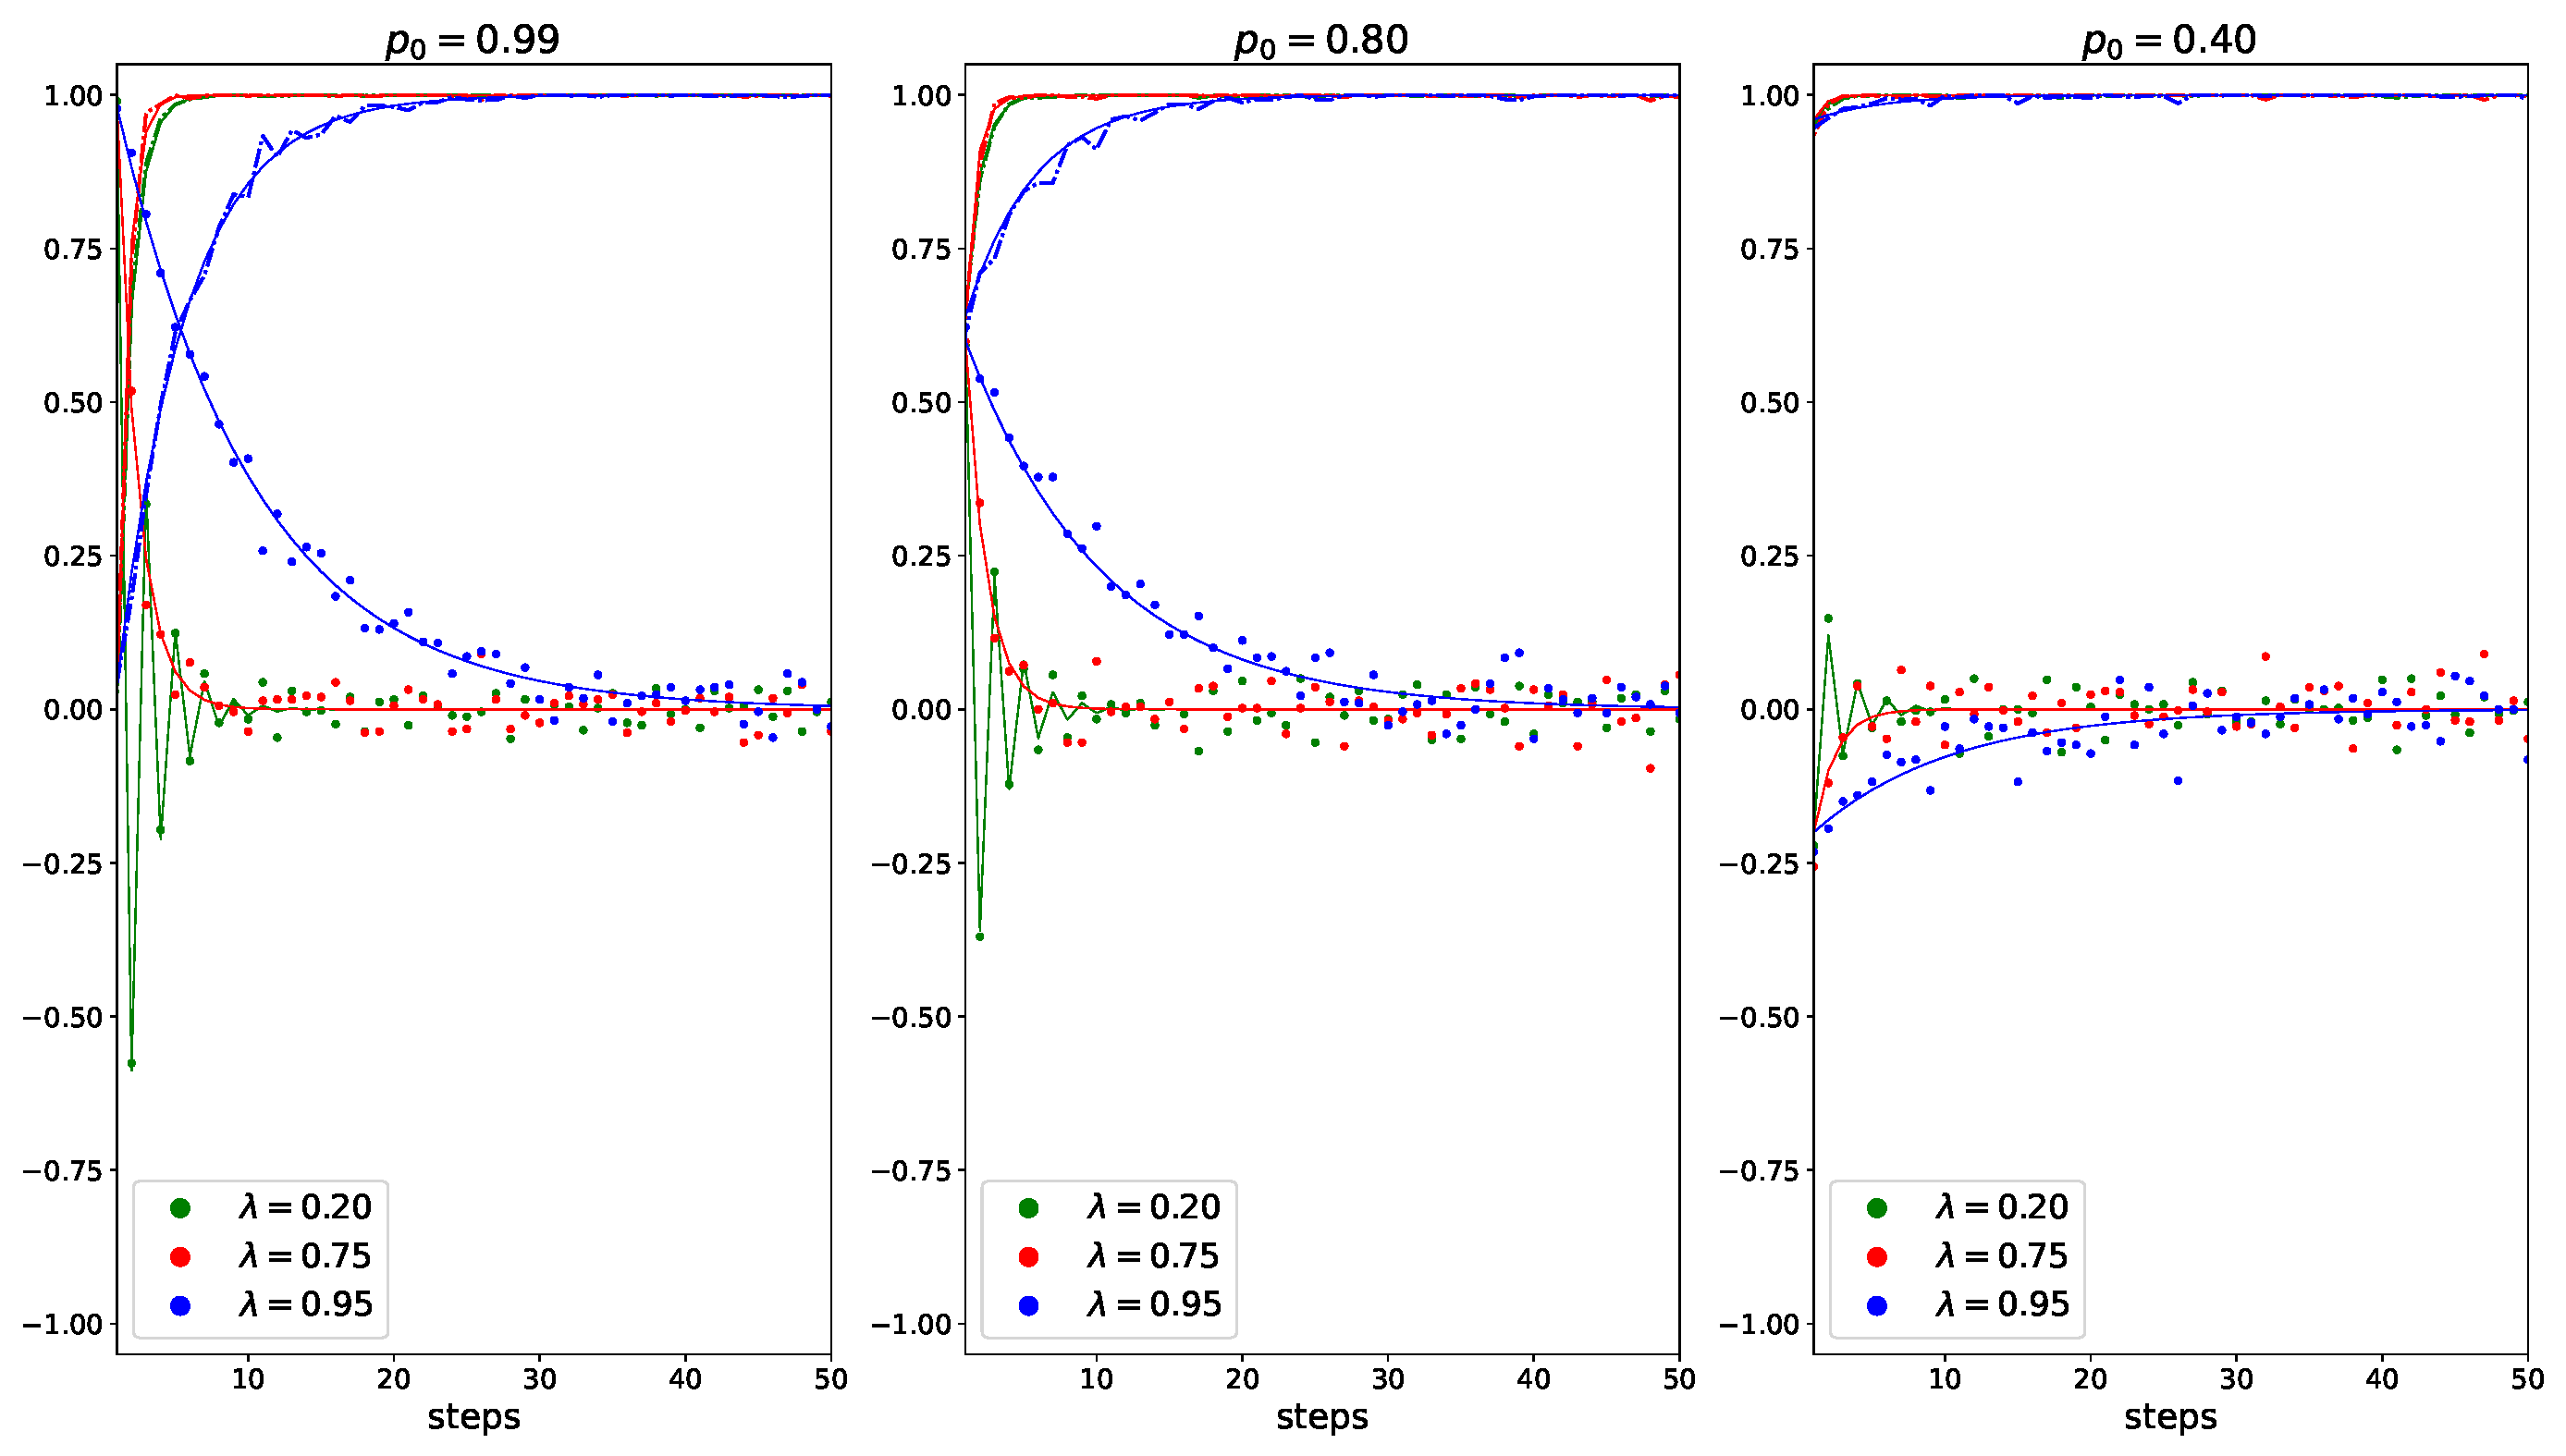
\includegraphics[width=1\textwidth]{../../simulations/e_step_1000_walks_50_steps_type_success_punished}
\end{frame}

\begin{frame}{Walk probabilities properties}

\[
EP_{t}=(2\lambda-1)^{t}p_{0}+\frac{1-(2\lambda-1)^{t}}{2},
\]
\[
\lim_{t\to+\infty}EP_{t}=\frac{1}{2}.
\]
\[
Var\,P_{t}=(3\lambda^{2}-2\lambda)^{t}p_{0}^{2}+\sum_{i=0}^{t-1}K(i;p_{0},\lambda)(3\lambda^{2}-2\lambda)^{t-1-i}-k(t;p_{o},\lambda)^{2},
\]
\[
\lim_{t\to+\infty}Var\,P_{t}=\frac{\frac{1}{2}(1-\lambda^{2})}{-3\lambda^{2}+2\lambda+1}-\frac{1}{4}.
\]

\end{frame}
%
\begin{frame}{Example - RW probabilities}

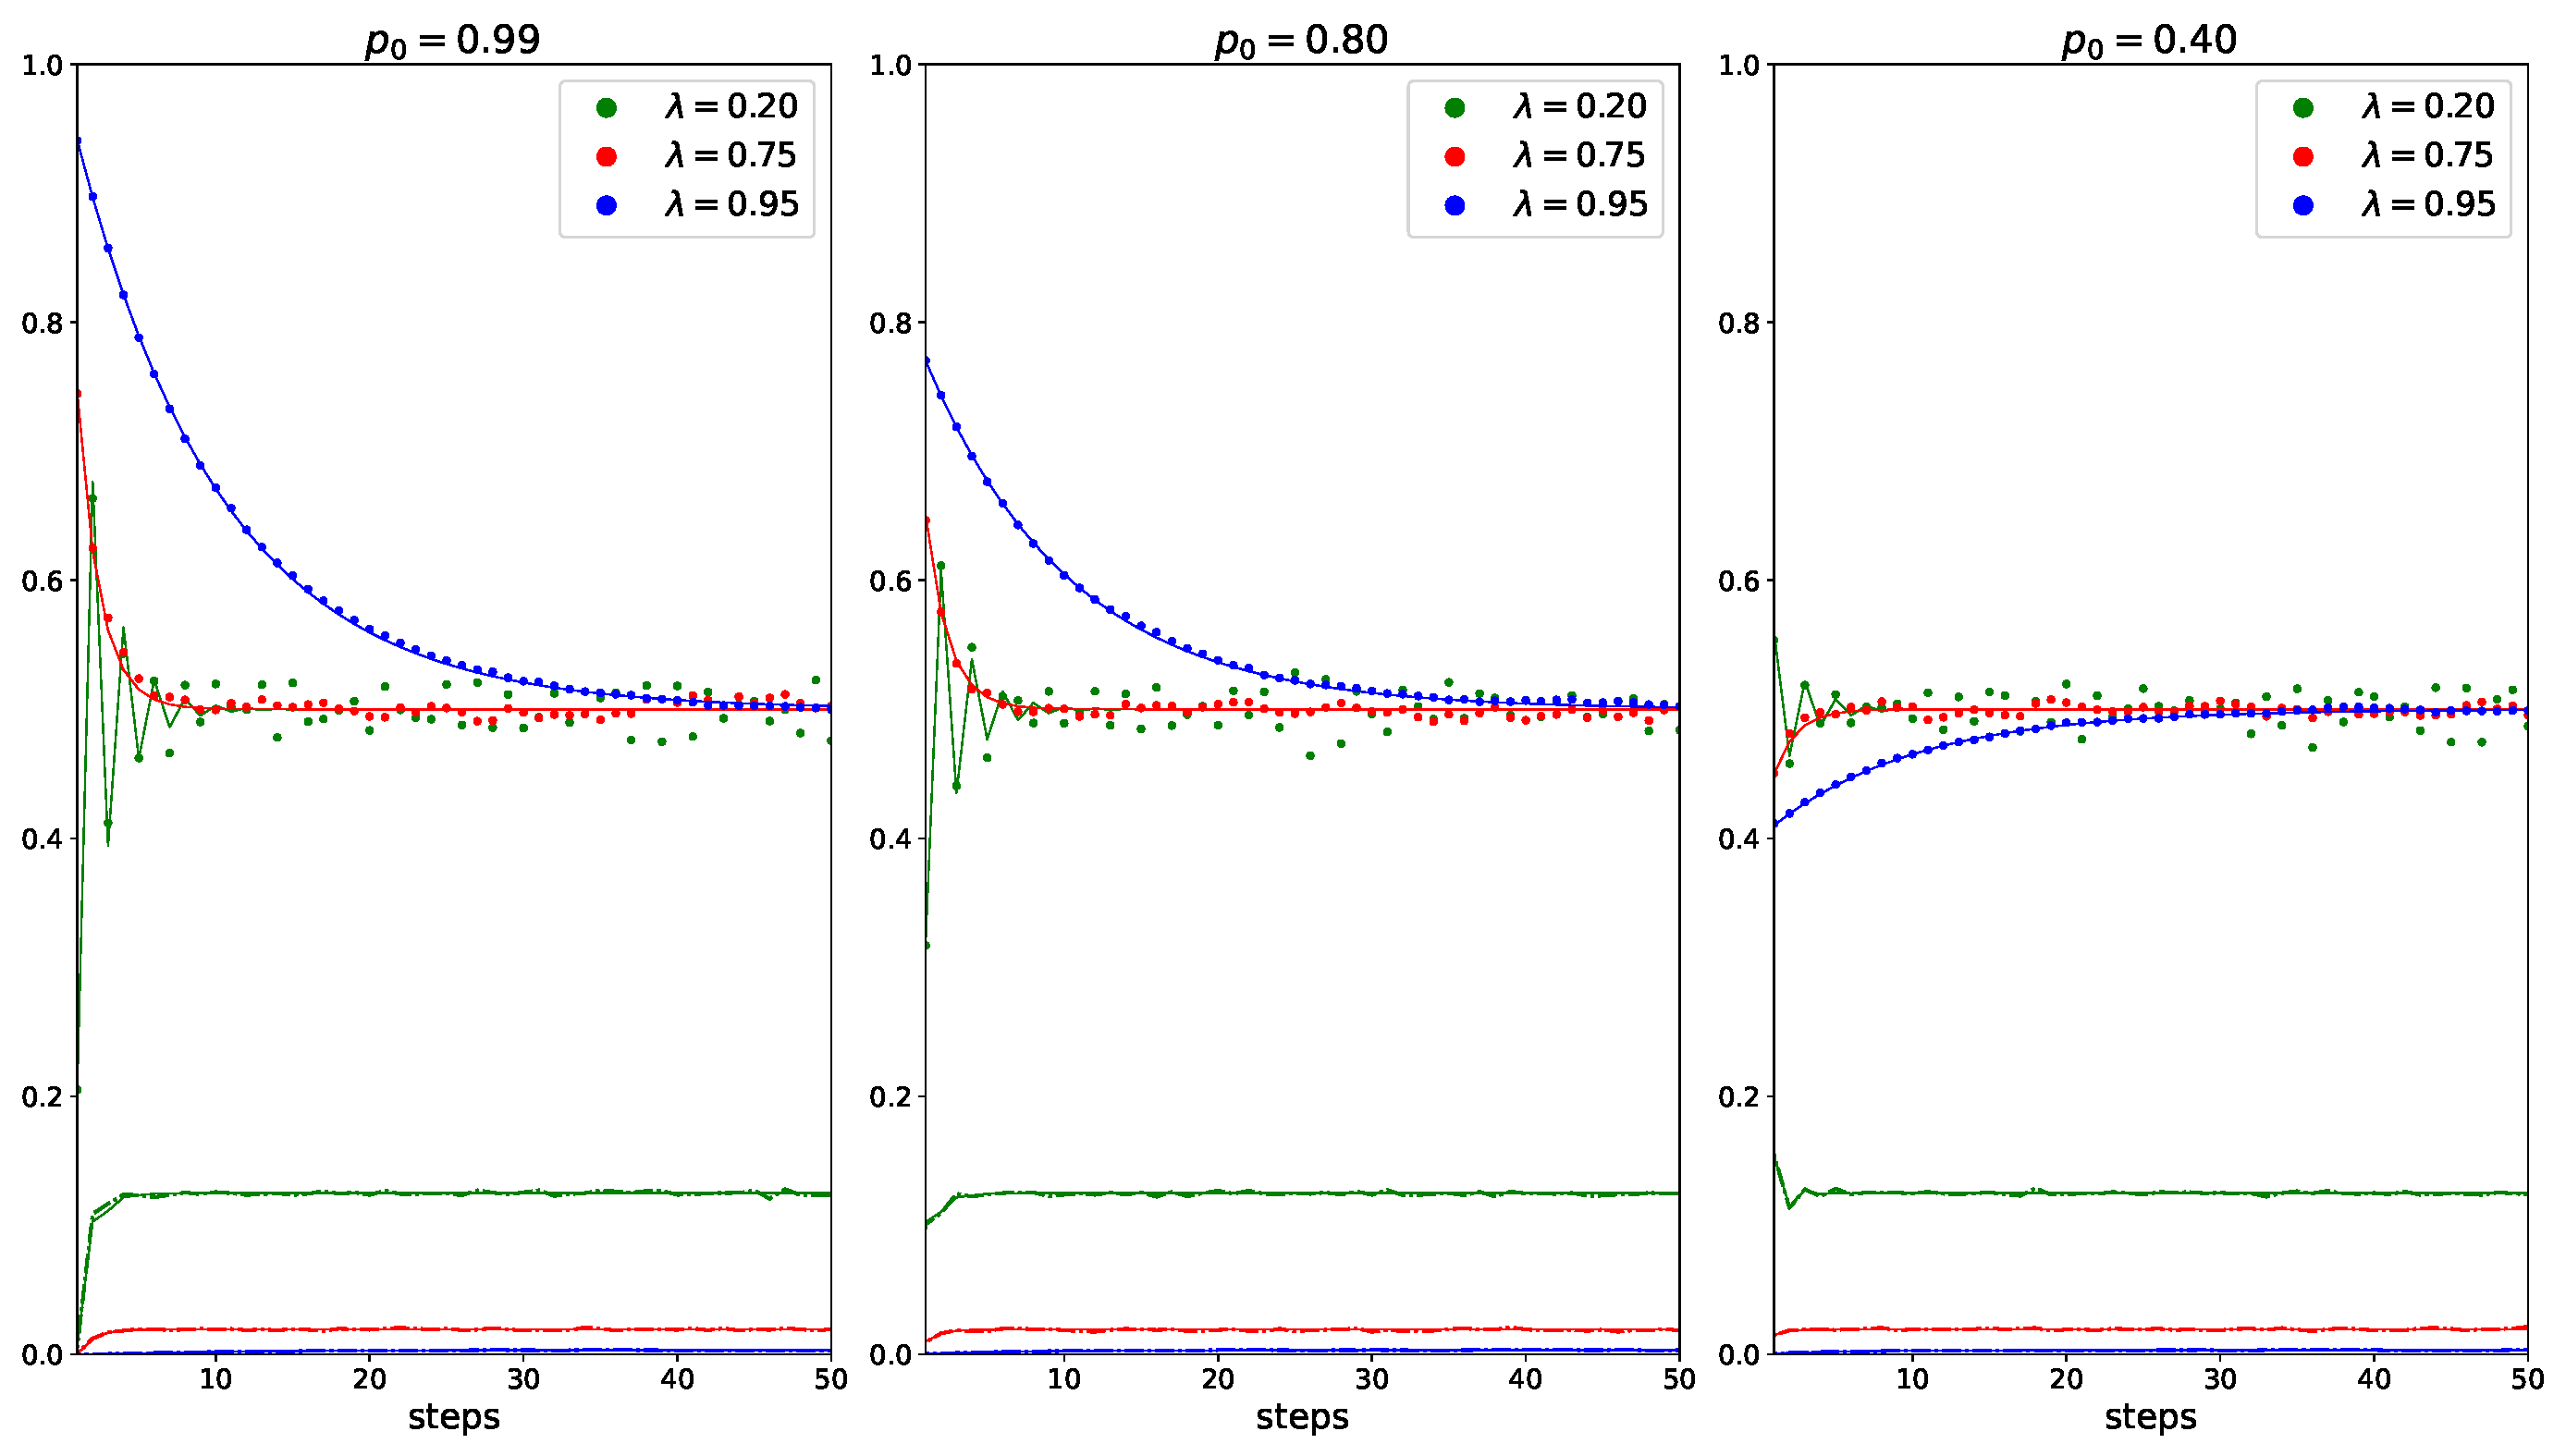
\includegraphics[width=1\textwidth]{../../simulations/e_probability_1000_walks_50_steps_type_success_punished}
\end{frame}
%
\begin{frame}{Walk position properties}

\[
ES_{t}=S_{0}+(2p_{0}-1)\frac{1-(2\lambda-1)^{t}}{2(1-\lambda)},
\]
\[
\lim_{t\to+\infty}ES_{t}=S_{0}+\frac{(2p_{0}-1)}{2(1-\lambda)}.
\]
\[
Var\,S_{t}=t+4\sum_{i=0}^{t-1}\sigma(i;p_{0},0,\lambda)-a(t;p_{0},\lambda),
\]
\[
\lim_{t\to+\infty}Var\,S_{t}=c_{1}(p_{0},\lambda)t+c_{2}(p_{0},\lambda).
\]

\end{frame}
%
\begin{frame}{Example - RW position}

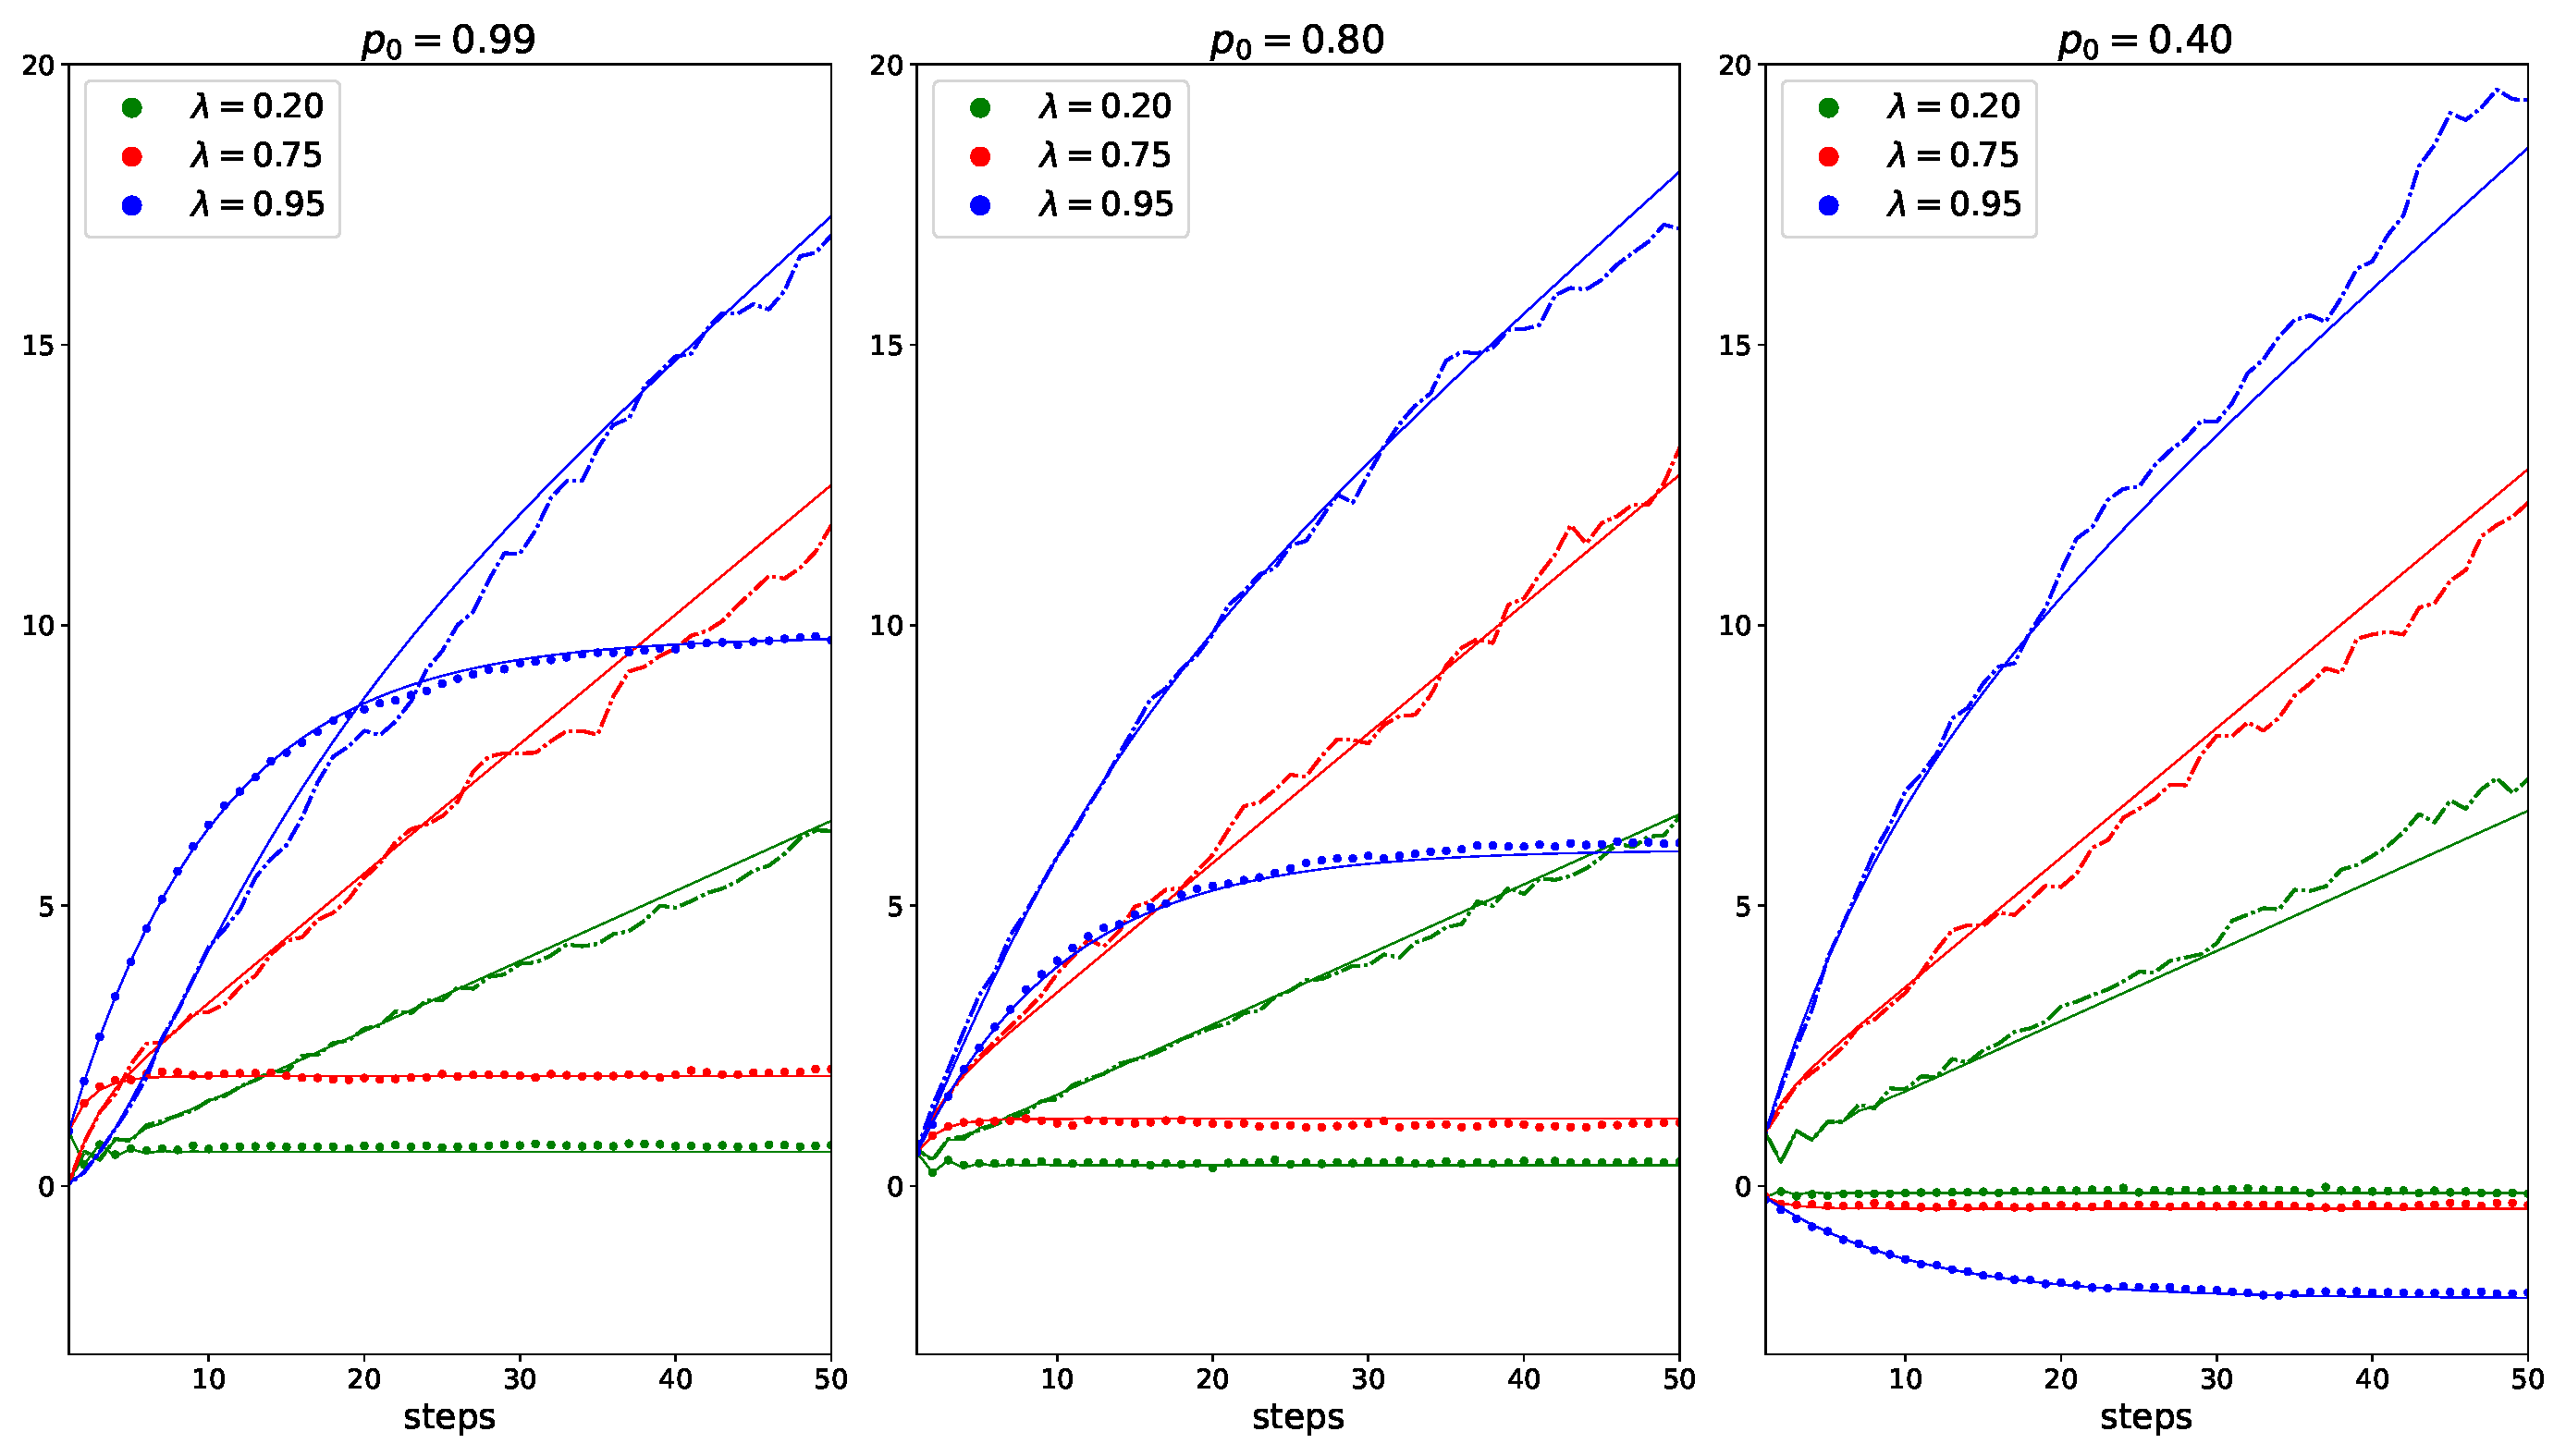
\includegraphics[width=1\textwidth]{../../simulations/e_position_1000_walks_50_steps_type_success_punished}
\end{frame}
%
\begin{frame}{Success rewarding model}

\[
EX_{t}=2p_{0}-1,
\]
\[
Var\,X_{t}=4p_{0}(1-p_{0}),
\]
\[
EP_{t}=p_{0},
\]
\[
Var\,P_{t}=(2\lambda-\lambda^{2})^{t}p_{0}^{2}+p_{0}(1-\lambda)^{2}\sum_{i=0}^{t-1}(2\lambda-\lambda^{2})^{i}-p_{0}^{2},
\]
\[
ES_{t}=S_{0}+t(2p_{0}-1),
\]
\[
Var\,S_{t}=4p_{0}(1-p_{0})t^{2}+a(p_{0},\lambda)t-a(p_{0},\lambda)\frac{1-(2\lambda-\lambda^{2})^{t}}{(1-\lambda)^{2}}.
\]

\end{frame}
%
\begin{frame}{Two-parameter model}
\begin{itemize}
\item Two parameters $\lambda$, each affecting one direction of the walk.
\item Again two variants - success punishing and success rewarding
\item<1-> $\frac{1}{2}[(1+X_{i})\lambda_{0}P_{i-1}+(1-X_{i})(1-\lambda_{1}(1-P_{i-1}))]$
\begin{itemize}
\item<1-> Two parameter success punishing model \medskip{}
\end{itemize}
\item<1-> $\frac{1}{2}[(1-X_{i})\lambda_{0}P_{i-1}+(1+X_{i})(1-\lambda_{1}(1-P_{i-1}))]$
\begin{itemize}
\item<1-> Two parameter success rewarding model 
\end{itemize}
\end{itemize}
\end{frame}
%
\begin{frame}{Example - two-parameter model}

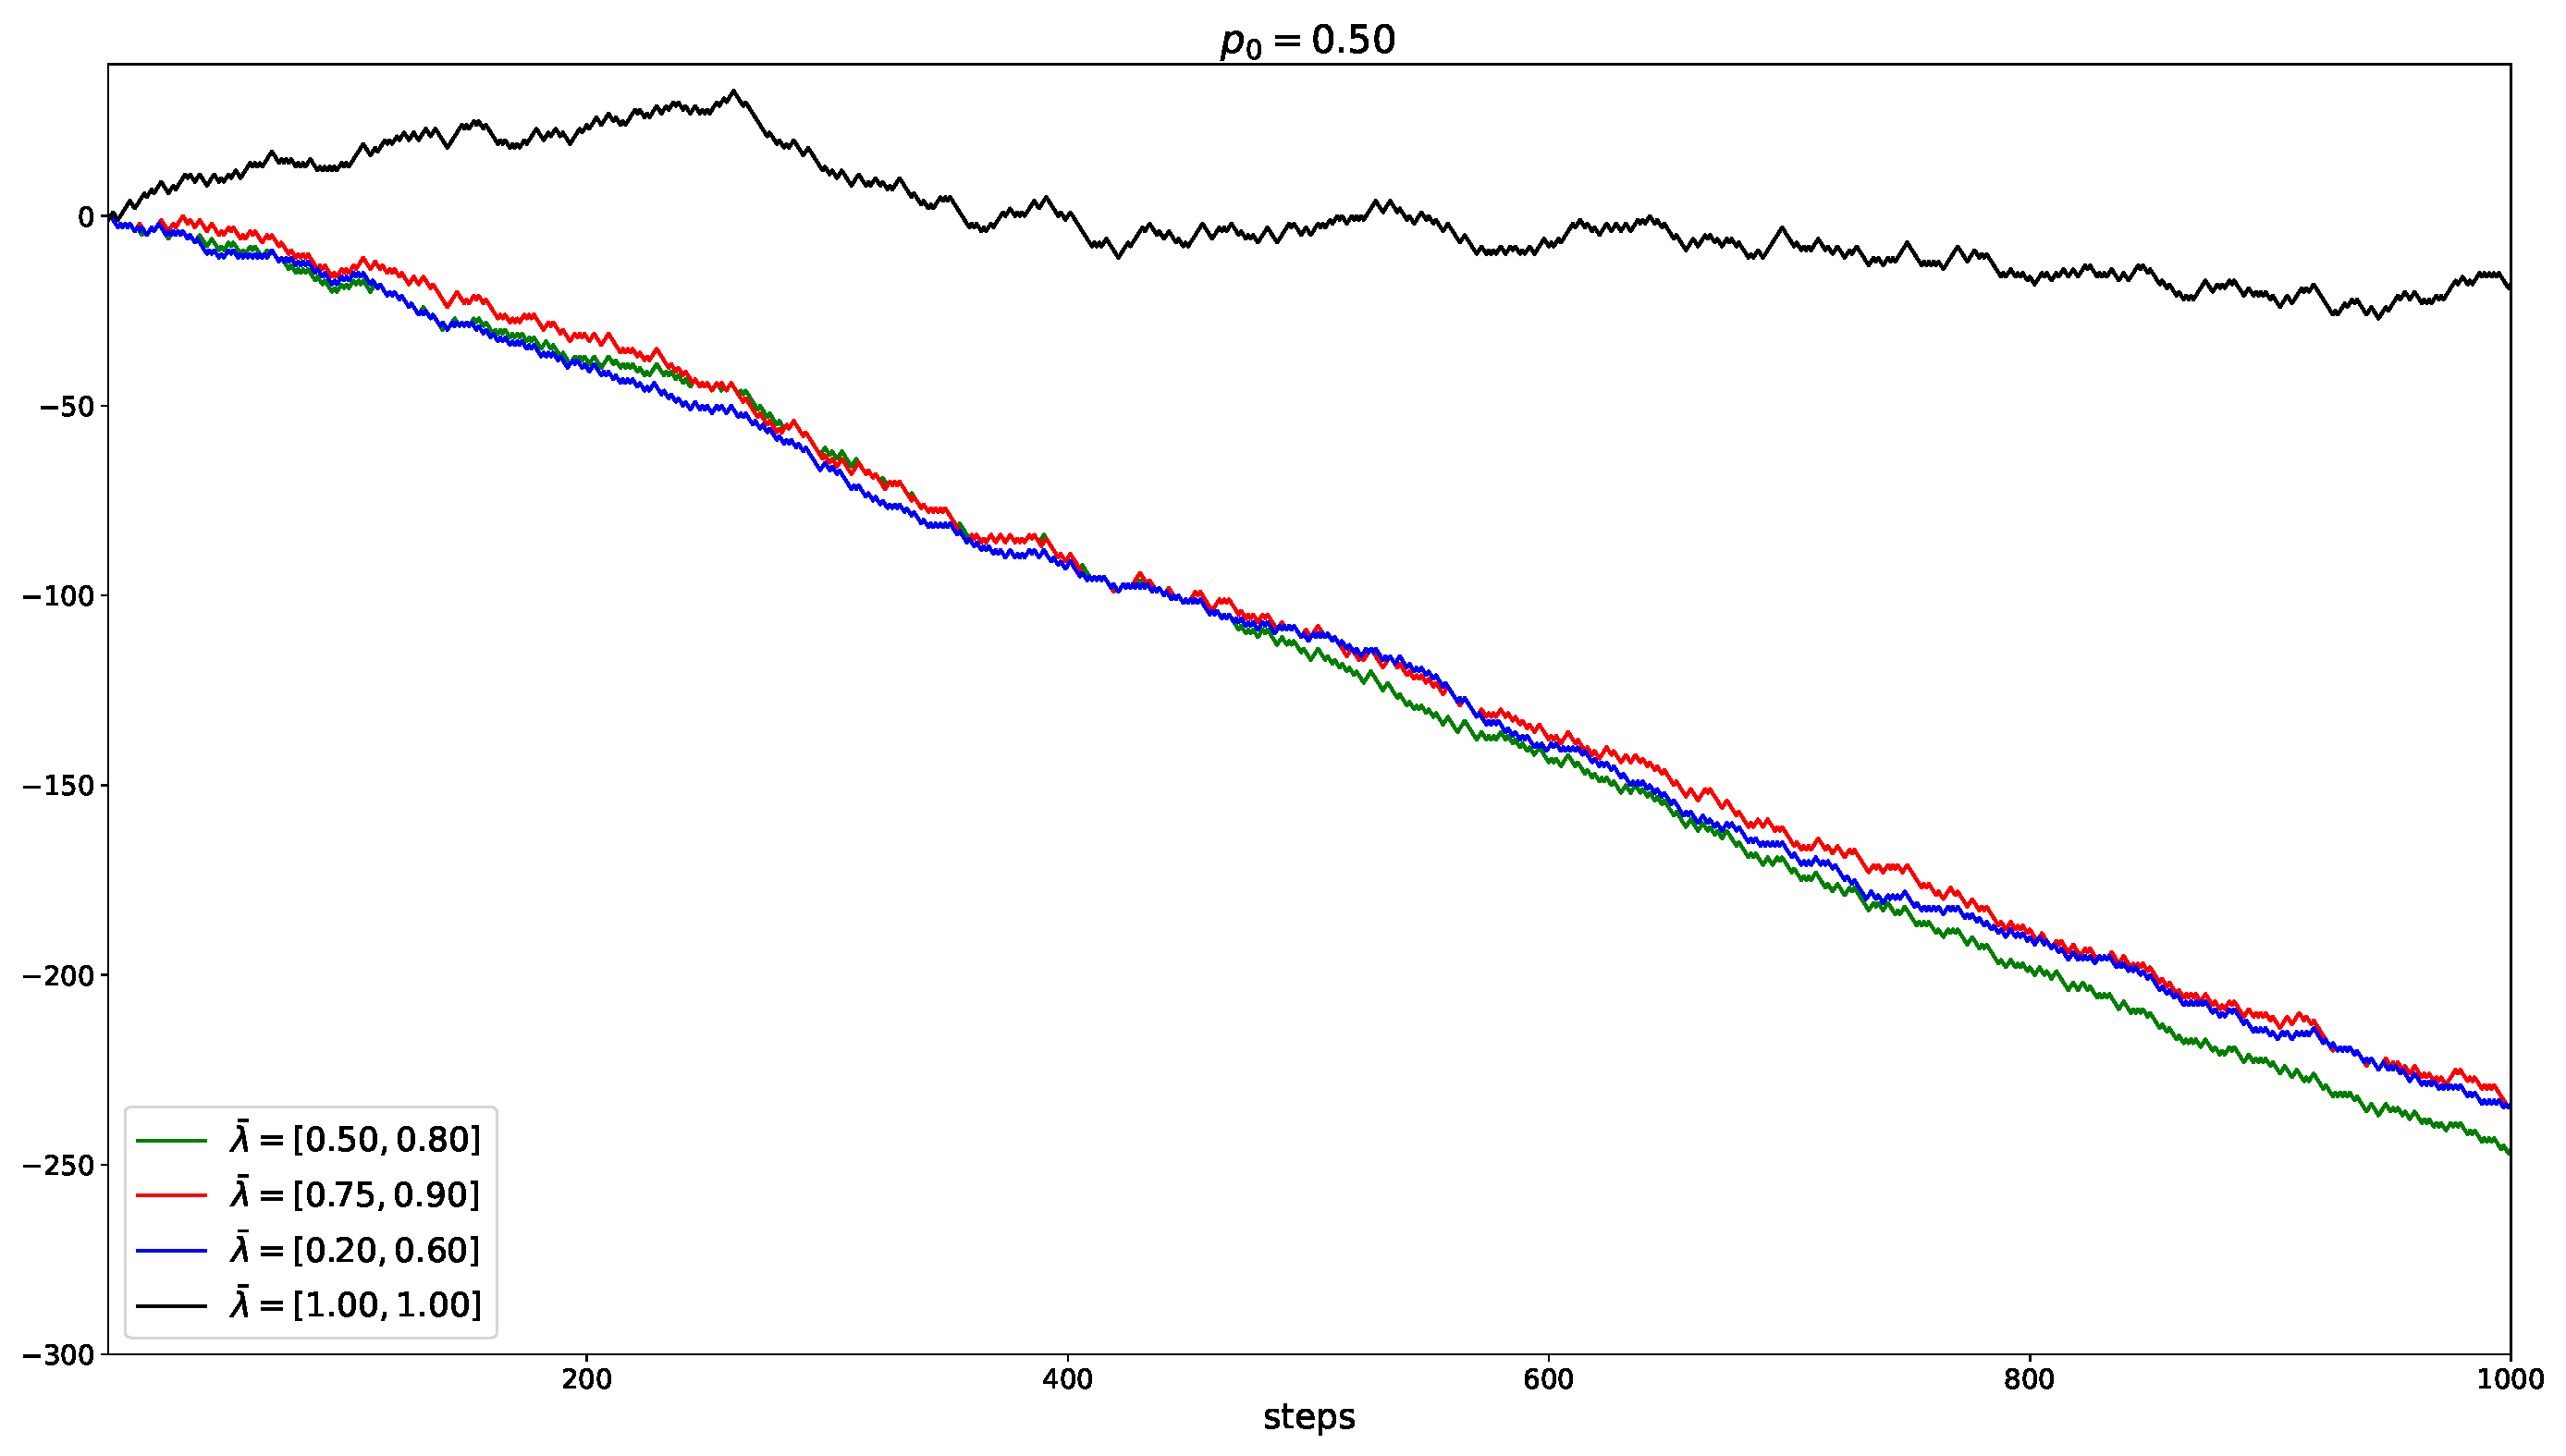
\includegraphics[width=1\textwidth]{../../simulations/single_walk_1000_steps_type_success_punished_two_lambdas}
\end{frame}
%
\begin{frame}{Model fitting}
\begin{itemize}
\item Find $\overrightarrow{\lambda}$ with known $p_{0}$, model type
\item Find $p_{0}$ with known $\overrightarrow{\lambda}$, model type
\item Find $p_{0},\,\overrightarrow{\lambda}$ with known model type
\begin{itemize}
\item Using maximal likelihood estimate \& numerical optimization
\end{itemize}
\item Find model type without any prior knowledge
\begin{itemize}
\item Using Akaike information criterion \& numerical optimization
\end{itemize}
\end{itemize}
\end{frame}
%
\begin{frame}{Real life application}
\begin{itemize}
\item Success rewarding model well suited for modelling tennis matches
\item Model trained on 2009 - 2018 men Grand Slam tournaments
\item Model applied on 2019 US Open
\begin{itemize}
\item Live betting against bookmaker
\item $0.52$ units total necessary bankroll
\item $2.24$ units total profit $\rightarrow$ $430\%$ ROI
\item Only 128 placed bets
\end{itemize}
\end{itemize}
\end{frame}
%
\begin{frame}{Summary}
\begin{itemize}
\item A specific model of a random walk with memory
\item Model properties derived
\item Application shows big future potencial of the model
\item Possible applications in a set of real life scenarios
\end{itemize}
\end{frame}

\end{document}
